% !TEX encoding = UTF-8
% !TEX program = pdflatex
% !TEX root = relazione.tex
% !TeX spellcheck = it_IT

% ESEMPI
\section{Esempi}\label{sec:esempi}
Dopo aver fatto una panoramica su cosa viene analizzato di un'immagine, in questa sezione verranno presentati alcuni esempi di utilizzo.
Sono state quindi individuate alcune funzionalità comuni a tutte le piattaforme: riconoscimento oggetti e ambientazione, riconoscimento di volti (singolo e con più volti).
%%
\subsection{Riconoscimento oggetti e ambientazione}\label{subsec:riconscimento-oggetti-ambientazione}
% TODO
%%
\subsection{Riconoscimento di un volto}\label{subsec:riconscimento-singolo-volto}
In questo confronto lo scopo era quello di verificare le caratteristiche del volto (\textit{landmark}) che l'API era in grado di riconsoscere in un ambiente semplice;
per questo motivo è stata scelta un'immagine di un primo piano di una ragazza\footnote{I diritti dell'immagine sono dei rispettivi proprietari.}.
Come si può notare dai risultati in Figura~\ref{fig:riconscimento-singolo-volto}, tutte le API hanno riconosciuto e identificato correttamente il volto e, a parte
il servizio offerto da IBM, diversi elementi di questo.
Il migliore di questi sembrerebbe essere le API di Google che, tuttavia, non fornisce indicazioni sulla persona specifica (età, sesso).
\begin{figure}[!h]
\begin{center}
	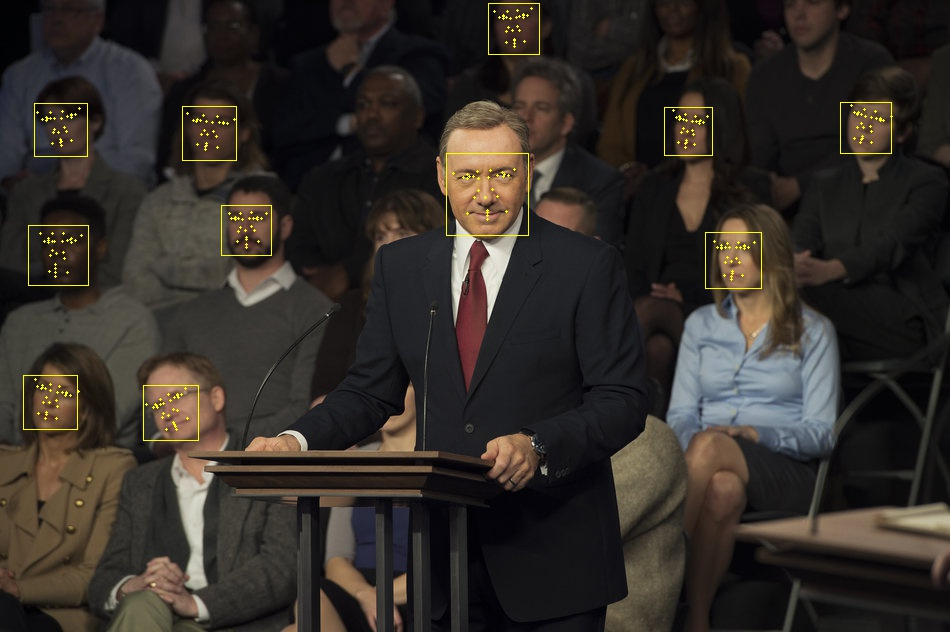
\includegraphics[width=200px,height=282px]{riconoscimento-viso-1/microsoft.jpg}
	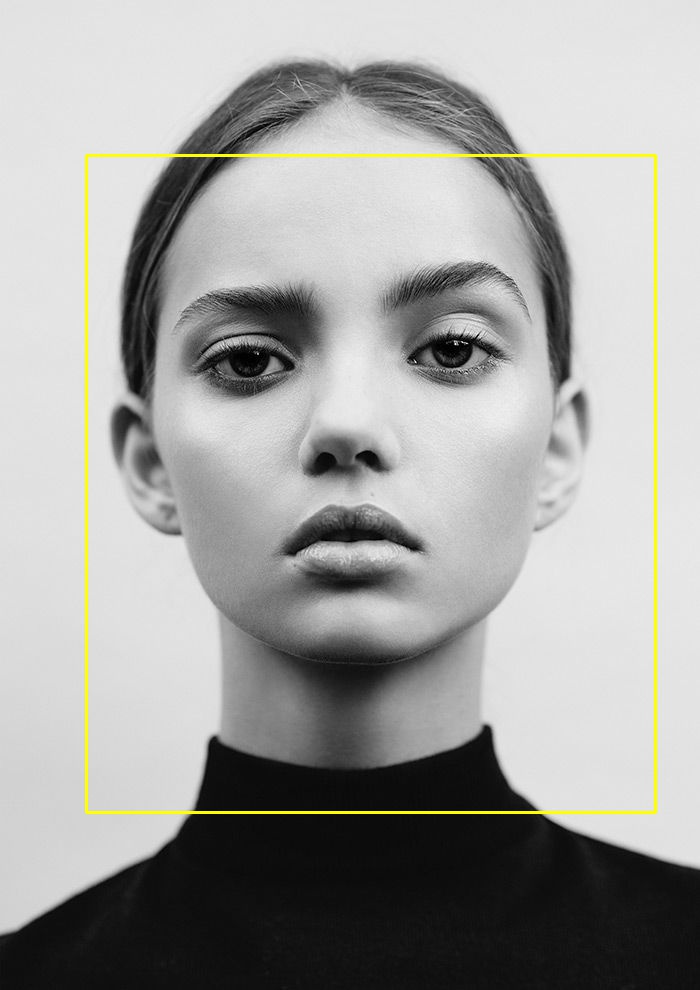
\includegraphics[width=200px,height=282px]{riconoscimento-viso-1/ibm.jpg}
	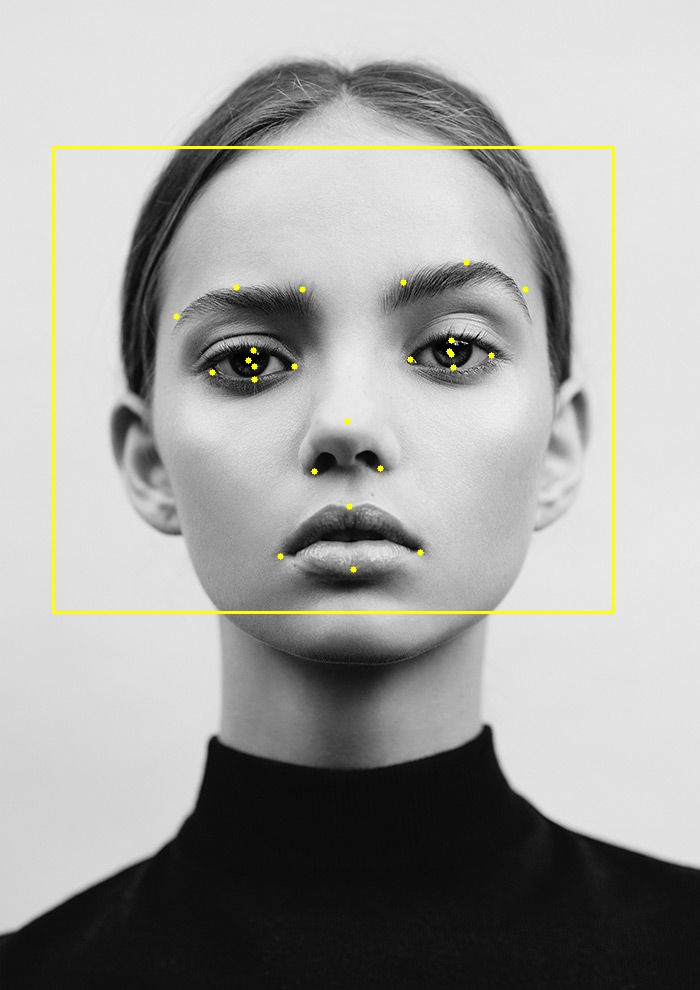
\includegraphics[width=200px,height=282px]{riconoscimento-viso-1/amazon.jpg}
	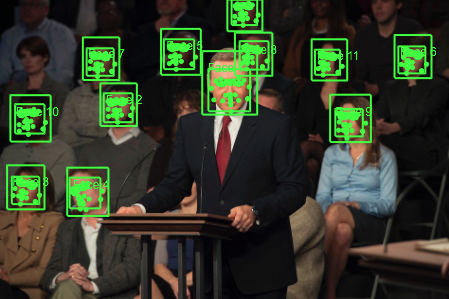
\includegraphics[width=200px,height=282px]{riconoscimento-viso-1/google.png}
{\scriptsize \caption{Riconscimento di un singolo volto utilizzando le API di(da sinistra): Microsoft, IBM, Amazon, Google. (Fonte: \url{http://eddienew.com})}
\label{fig:riconscimento-singolo-volto}}
\end{center}
\end{figure}
%
\subsection{Riconoscimento di più volti}\label{subsec:riconscimento-piu-volti}
%
